\documentclass{beamer}

\usetheme[progressbar=frametitle]{metropolis}
\setbeamertemplate{frame numbering}[fraction]

\title{House Price Predictions, Intervals, and Combinations}
\subtitle{A Study for Perth in Australia}
\author{Zhuoran (Thomas) Zhang}
\institute{University of Aberdeen \& Curtin University}
\date{\today}

\begin{document}

\AtBeginSection[]
{
  \begin{frame}
    \frametitle{Table of Contents}
    \tableofcontents[currentsection]
  \end{frame}
}

\AtBeginSubsection[]
{
  \begin{frame}
    \frametitle{Table of Contents}
    \tableofcontents[currentsubsection]
  \end{frame}
}

\begin{frame}
\titlepage
\end{frame}

\section{Introduction}

\begin{frame}[t]{Introduction}
\begin{block}{What we did?}
\vspace{0.5em}
Automated Valuation Models (AVM), which could provide estimated house price by giving specific variables about properties.
\end{block}

\begin{block}{Why?}
\begin{enumerate}
\item Housing Automated Valuation Service (AVS).
\item Mortgage underwriting, properties refinancing for banking service.
\item Tax assessment; Risk assessment of loan pools.
\end{enumerate}
\end{block}

\end{frame}

\begin{frame}[t]{Introduction}

\begin{block}{Research Questions}
\begin{enumerate}
\item Which model is the best or most accurate to provide housing automated valuation service?
\item What is the uncertainty of these predictions from models?
\item Is using the single best model better than models cooperation?
\end{enumerate}
\end{block}

\begin{block}{How?}
\begin{enumerate}
\item Examining models in full samples and rolling windows samples. The Performance of models will be compared.
\item Calculating the predict interval of each observation by quantile measures.
\item Trying the forecast combination (or model averaging).
\end{enumerate}
\end{block}

\end{frame}

\begin{frame}[t]{Literatures}

\begin{block}{Main Four}
\begin{enumerate}
\item \textbf{Automated Valuation Modelling: A Specification Exercise}. (2013). R. Schulz; M, Wersing and A, Werwatz.
\item \textbf{An Introduction to Statistical Learning with Applications in R}. (2013). G, James; D, Witten and T, Hastie.
\item \textbf{Semi-parametric Regression with R}. (2018). J, Harezlak; D, Ruppert and M, Wand. 
\item \textbf{Model Averaging and Its Use in Economics}. (2020). Mark F. J. Steel. 
\end{enumerate}
\end{block}

\end{frame}

\section{Data}

\begin{frame}[t]{Real Estate Data in Perth, Australia}

\begin{columns}[onlytextwidth]
\column{0.5\textwidth}
\begin{block}{Basic Info}
\vspace{0.5em}
\begin{itemize}
\item \textcolor{blue}{Landgate} is our data provider, the Western Australian Land Information Authority.
\item Research Period: \textbf{1989.01.01 -- 2019.12.31}.
\item No. of Observations: \textbf{755,670} house transactions in total.
\end{itemize}
\end{block}
\column{0.5\textwidth}
\begin{figure}
\caption{The Satellite Shot of Perth}
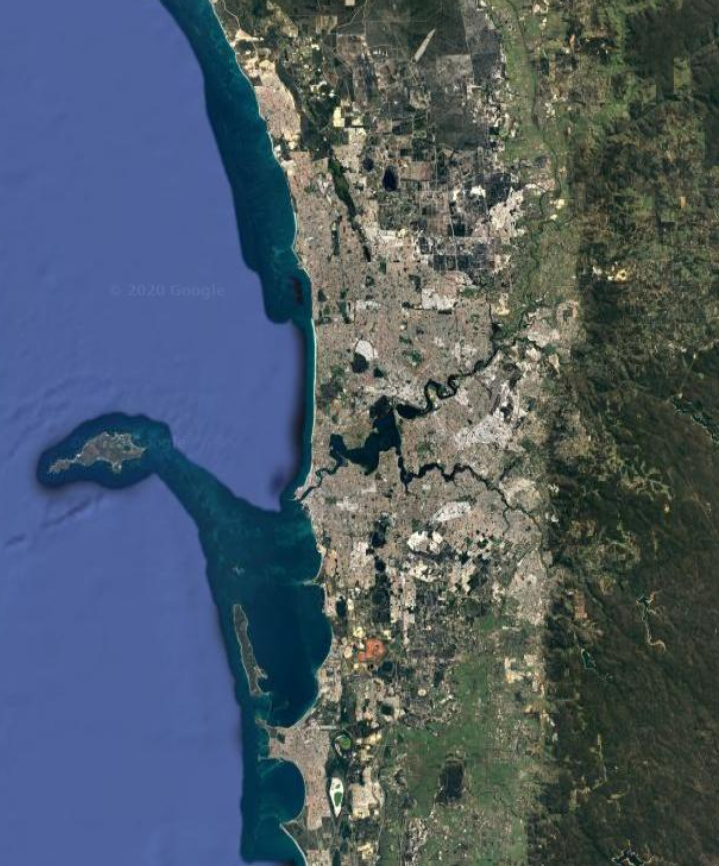
\includegraphics[scale=0.25]{perth}
\end{figure}
\end{columns}

\end{frame}

\begin{frame}[t]{Real Estate Data in Perth, Australia Cont'd}

\begin{block}{Available Variables}
\begin{itemize}
\item Transaction price and date.
\item Year of build and land area. 
\item Number of rooms and other facilities.
\item Location coordinates.
\end{itemize}
\end{block}

\begin{block}{Data Cleaning}
\begin{itemize}
\item Restrict between 1 and 6 bedrooms.
\item Restrict between 1 and 5 bathrooms. 
\item Restrict between 0 and 5 the other functional rooms.
\item Filter the typos and meaningless observations.
\end{itemize}
\end{block}

\end{frame}

\begin{frame}[t]{Real Estate Data in Perth, Australia Cont'd}

\begin{block}{}
\textbf{45,558} observations are cleaned. \textbf{710,112} observations in final data set.
\end{block}

\begin{table}
\caption{The Summary Statistics of Final Dataset}
\vspace*{-\baselineskip}
\scalebox{0.9}{
\begin{tabular}{lcccc}
		&Mean    &Std.Dev.&Min   &Max\\
\hline
Price &379,442 &431,851 &10,000 &50,000,000\\
Land Area &789.4 &560.3 &100 &10,000\\
Age &24.5 &20.2 &0 &135\\
Bedroom &3.3 &0.8 &1 &6\\
Bathroom &1.5 &0.6 &1 &5\\
Car Park &1.4 &0.8 &0 &5\\
Pool &0.15 &0.36 &0 &1\\
\end{tabular}}
\end{table}
\end{frame}

\section{Summary of Methodology}

\begin{frame}[t]{Models Summary}

\begin{block}{Parametric Group}
\begin{enumerate}
\item Basic Linear Model (\textbf{Model 1})
\item Linear Models with Three Estimators (Ridge, LASSO, Elastic-Net; \textbf{Model 2-4})
\item Polynomial Model with Power 10 (\textbf{Model 5})
\end{enumerate}
\end{block}

\begin{block}{Semi-parametric Group: Spline Models}
\begin{enumerate}
\item \textbf{Model 6}:
\begin{equation}
ln~price = Z\beta + f(z_{lon}, z_{lat}) + \epsilon.
\end{equation}
\item \textbf{Model 7}:
\begin{equation}
ln~price = Z\beta + f(z_{lon}, z_{lat}, z_{land area}) + \epsilon.
\end{equation}
\end{enumerate}
\end{block}

\end{frame}

\begin{frame}[t]{Models Summary (Cont'd)}

\begin{block}{Semi-parametric Group: Spline Models (Cont'd)}
\begin{enumerate}
\item[3.] \textbf{Model 8}
\begin{equation}
ln~price = Z\beta +f(z_{age}) + g(z_{lon}, z_{lat}) +  h(z_{land area}) + \epsilon.
\end{equation}
\item[4.] \textbf{Model 9}
\begin{equation}
ln~price = Z\beta + f(z_{age}) + g(z_{lon}, z_{lat}, z_{land area}) + \epsilon.
\end{equation}
\end{enumerate}
\end{block}


\begin{block}{Tree Based Group}
\begin{enumerate}
\item Regression Tree (\textbf{Model 10})
\item Random Forest (\textbf{Model 11}), Boosting (\textbf{Model 12})
\item Neutral Network (\textbf{Model 13})
\end{enumerate}
\end{block}
\end{frame}

\section{Analysis and Results}
\subsection{Full Sample Analysis and Results}

\begin{frame}[t]{Full Sample Analysis}

\begin{block}{Data Preparation}
\vspace{0.5em}
Training (497,081); Combination (106,515); Testing (106,516).
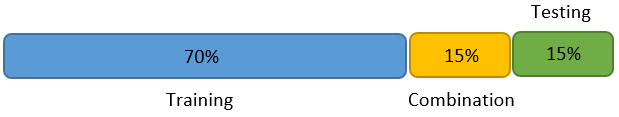
\includegraphics[scale=0.6]{data_partition}
\end{block}

\begin{block}{Tuning Parameters}
\begin{itemize}
\item Cross Validation (Regularization Estimators, Machine Learning).
\item Package \textit{caret} in R.
\end{itemize}
\end{block}
\end{frame}

\begin{frame}[t]{Full Sample Results}

\begin{table}
\caption{The Summary of Full Sample Results}
\scalebox{0.9}{
\begin{tabular}{lcccc}
Models &RMSE &MAPE &$<$1\% Relative &$<$5\% Relative\\
\hline
Model 1 &0.40120 &0.02268 &34,350 (32.25\%) &96,820 (90.90\%)\\
Model 2 &0.40638 &0.02305 &33,864 (31.79\%) &96,343 (90.45\%)\\
Model 3 &0.40131 &0.02267 &34,354 (32.25\%) &96,802 (90.88\%)\\
Model 4 &0.40234 &0.02274 &34,237 (32.14\%) &96,717 (90.80\%)\\
Model 5 &0.32370 &0.01735 &44,856 (42.11\%) &101,458 (95.25\%)\\
Model 6 &0.30260 &0.01585 &48,879 (45.89\%) &102,408 (96.14\%)\\
Model 7 &0.29673 &0.01549 &49,833 (46.78\%) &102,692 (96.41\%)\\
\end{tabular}}
\end{table}
\end{frame}


\begin{frame}[t]{Full Sample Results (Cont'd)}

\begin{table}
\caption{The Summary of Full Sample Results, Cont'd}
\scalebox{0.9}{
\begin{tabular}{lcccc}
Models &RMSE &MAPE &$<$1\% Relative &$<$5\% Relative\\
\hline
Model 8 &0.28991 &0.01485 &52,838 (49.61\%) &102,875 (96.58\%)\\
Model 9 &0.28832 &0.01473 &52,222 (49.03\%) &102,788 (96.50\%)\\
Model 10 &\textcolor{blue}{0.63833} &\textcolor{blue}{0.04027} &\textcolor{blue}{16,652 (15.63\%)} &\textcolor{blue}{73,685 (69.18\%)}\\
Model 11 &0.28931 &0.01423 &58,348 (54.78\%) &102,114 (95.87\%)\\
Model 12 &\textcolor{red}{0.25282} &\textcolor{red}{0.01211} &\textcolor{red}{63,653 (59.76\%)} &\textcolor{red}{103,607 (97.27\%)}\\
Model 13 &0.28041 &0.01398 &55,904 (52.48\%) &103,009 (96.71\%)\\
\end{tabular}}
\end{table}
\end{frame}

\begin{frame}[t]{Full Sample Results (Cont'd)}
\begin{figure}
\caption{Error Rates of Models}
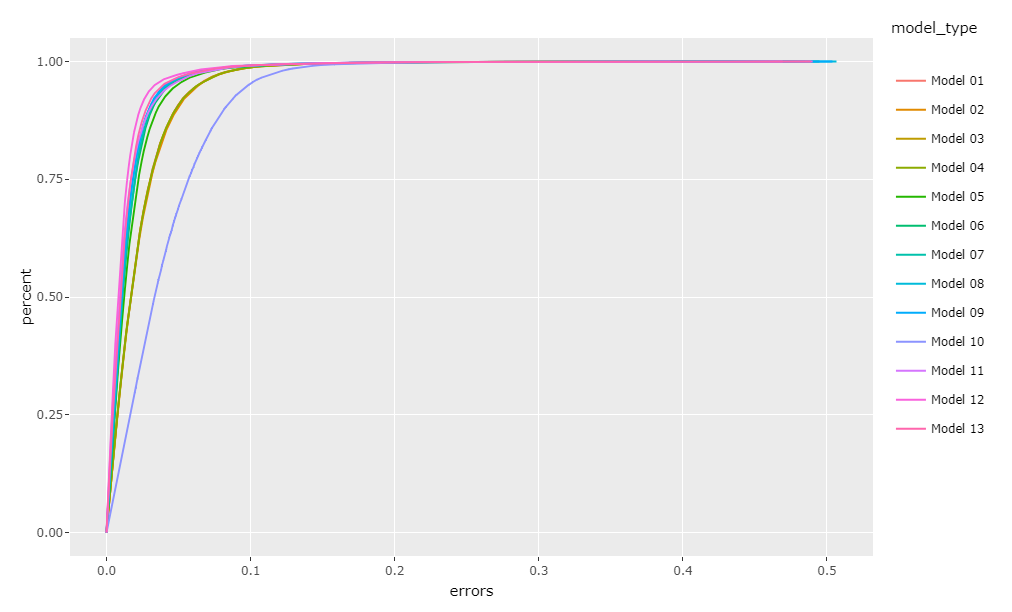
\includegraphics[scale=0.4]{figure10}
\end{figure}
\end{frame}

\begin{frame}[t]{Full Sample Results -- Models Comparison}

\begin{block}{Accuracy:}
\vspace{0.5em}
Parametric Group $<$ Semi-parametric Group $<$ Tree Based Group 
\end{block}

\begin{block}{Model Interpretability:}
\vspace{0.5em}
Tree Based Group $<$ Parametric Group $<$ Semi-parametric Group\\
\vspace{0.5em}
\begin{itemize}
\item \textbf{Tree Based Group}: Black box process; Predictions.\\

\item \textbf{Parametric Group}: Clear and easy process; Parameters, Predictions.\\

\item \textbf{Semi-parametric Group}: Clear but complex process; Some parameters, Predictions, \textbf{Graphs}. 
\end{itemize}
\end{block}
\end{frame}

\begin{frame}[t]{Full Sample Results -- Models Comparison Cont'd}
\begin{columns}[onlytextwidth]
\column{0.5\textwidth}
\begin{figure}
\caption{Price Predictor Contours (700 $m^2$ Land Area)}
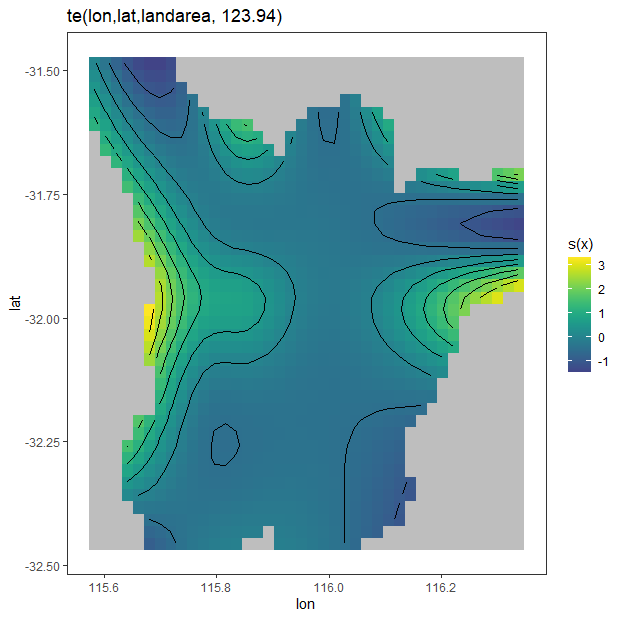
\includegraphics[scale=0.3]{spline_700m2}
\end{figure}
\column{0.5\textwidth}
\begin{figure}
\caption{Price Predictor Contours (1000 $m^2$ Land Area)}
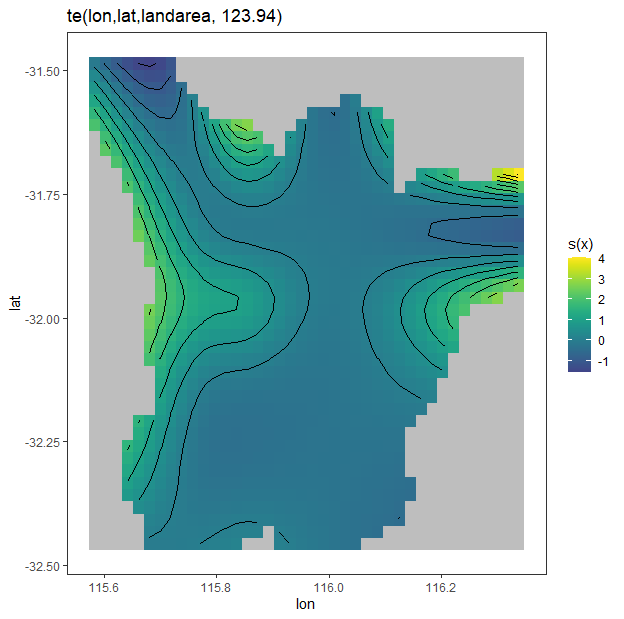
\includegraphics[scale=0.3]{spline_1000m2}
\end{figure}
\end{columns}
\end{frame}

\begin{frame}[t]{Full Sample Results -- Prediction Intervals}

\begin{table}
\caption{The Summary of Prediction Intervals ($95\%$)}
\vspace*{-\baselineskip}
\begin{tabular}{lccccccc}
Method &Mean Width &S.D. of Width &Rate within Interval\\
\hline
Linear         &0.1191 &0.0257 &94.97\%\\
Spline         &0.0887 &0.0222 &95.69\%\\
Boosting       &\textcolor{red}{0.0730} &0.0316 &\textcolor{blue}{93.91\%}\\
Random Forest  &\textcolor{blue}{0.1230} &0.0297 &\textcolor{red}{97.26\%}\\
Neural Network &0.0808 &0.0264 &94.76\%\\
Averaging      &\underline{0.0969} &0.0202 &\underline{97.15\%}\\
\end{tabular}
\end{table}

\begin{columns}[onlytextwidth]
\column{0.5\textwidth}
\begin{equation}
Width = \frac{Upper - Lower}{Market Value}
\end{equation}
\column{0.5\textwidth}
\begin{equation}
Rate = \frac{No.~fall~in~interval}{Total~No.}
\end{equation}
\end{columns}
\end{frame}

\begin{frame}[t]{Full Sample Results -- Prediction Intervals Cont'd}
\vspace*{-\baselineskip}
\begin{columns}[onlytextwidth]
\column{0.5\textwidth}
\begin{figure}
\caption{Falling in Interval Versus Width (Random Forest)}
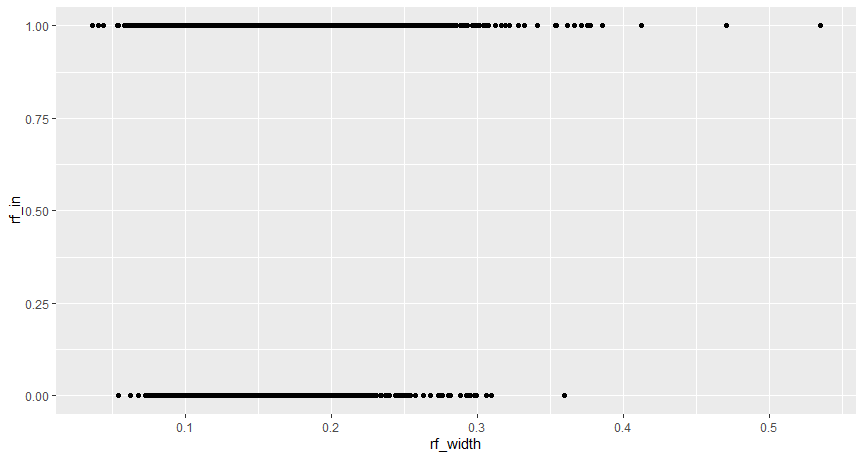
\includegraphics[scale=0.2]{rf_width_plot}
\end{figure}
\vspace*{-\baselineskip}
\begin{figure}
\caption{Falling in Interval Versus Width (Boosting)}
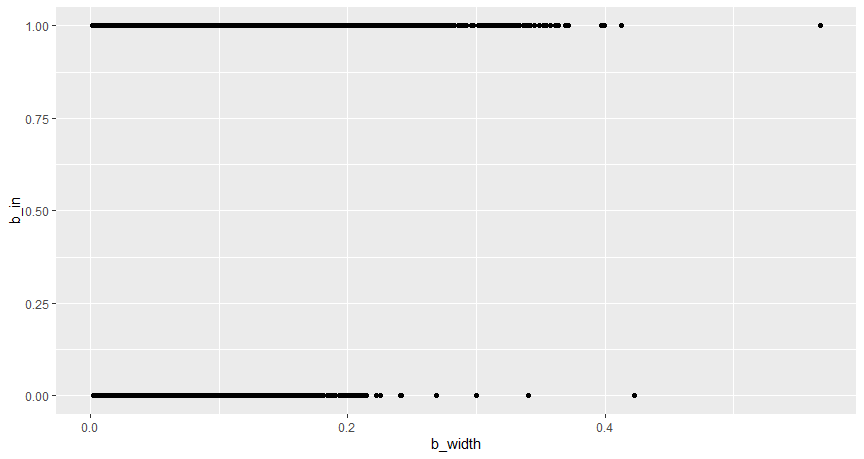
\includegraphics[scale=0.2]{b_width_plot}
\end{figure}

\column{0.5\textwidth}
\vspace*{-\baselineskip}
\begin{figure}
\caption{Falling in Interval Versus Width (Averaging)}
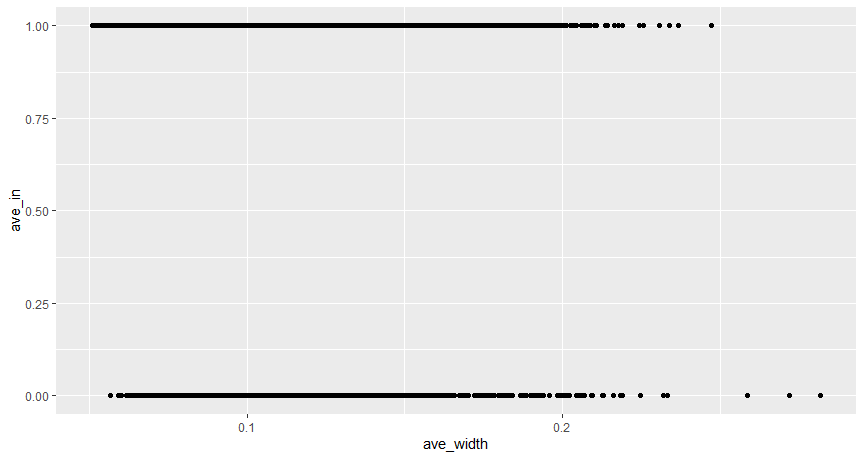
\includegraphics[scale=0.2]{ave_width_plot}
\end{figure}
\vspace*{-\baselineskip}
\begin{block}{}
\vspace*{-\baselineskip}
\begin{itemize}
\item When the confidence of prediction intervals are 95\%, the predictions should have 5\% chance to fall out of the intervals no matter how wide the intervals are.
\end{itemize}

\end{block}

\end{columns}

\end{frame}

\begin{frame}[t]{Full Sample Combination}
\begin{block}{Combination Methods}
\vspace{0.5em}
Linear Regression Combination; Quantile Regression Combination; Averaging Combination.
\end{block}

\begin{block}{Forecasts Selection}
\vspace{0.5em}
All Variables; Best Four Models (9, 11, 12 \& 13); LASSO Selection (11, 12 \& 13).
\end{block}

\begin{block}{Adding Updated Past Sale Price (Extension)}
\vspace{0.5em}
Past prices are updated by local housing price index, then they will be added into combination. 
\end{block}

\begin{block}{Example:}
\vspace*{-\baselineskip}
\begin{equation}
ln~price = c + (Past~Price) + w_1 forecast_1 + \cdots + w_{13} forecast_{13} + \varepsilon.
\end{equation}
\end{block}

\end{frame}

\begin{frame}[t]{Full Sample Combination (Cont'd)}

\begin{table}
\caption{The Results of Combinations and Their Extension}
\scalebox{0.58}{
\begin{tabular}{llccccccc}
Method &Variables & &\multicolumn{2}{c}{With Past Sale Prices} &\multicolumn{2}{c}{Without Past Sale Prices} &\multicolumn{2}{c}{Overall}\\\cline{4-9}
 & &  &Extension &Origin  &Extension &Origin &Extension &Origin\\
\hline
Linear     &All &RMSE &0.23708 &0.23907 &0.27661 &0.27678 &0.24909 &0.25050\\ 
       	   &Forecasts &MAPE &0.01107 &0.01122 &0.01357 &0.13576 &0.01179 &0.01190\\\cline{2-9}
           &Best &RMSE &0.23783 &0.23984 &0.27735 &0.27760 &0.24984 &0.25128\\
Regression &Four &MAPE &0.01111 &0.01126 &0.01360 &0.01359 &0.01182 &0.01193\\\cline{2-9}
		   &LASSO &RMSE &0.23791 &0.23991 &0.27747 &0.27769 &0.24993 &0.25136\\
           &Selection &MAPE &0.01110 &0.01126 &0.01359 &0.01359 &0.01182 &0.01193\\
\hline
Quantile   &All &RMSE &0.23803 &0.23993 &0.27716 &0.27764 &0.24991 &0.25135\\
           &Forecasts &MAPE &0.01102 &0.01115 &0.01347 &0.01352 &0.01172 &0.01183\\\cline{2-9}
           &Best &RMSE &0.23867 &0.24054 &0.27797 &0.27842 &0.25061 &0.25202\\
Regression &Four &MAPE &0.01107 &0.01120 &0.01351 &0.01356 &0.01177 &0.01188\\\cline{2-9}
           &LASSO &RMSE &0.23865 &0.24051 &0.27796 &0.27840 &0.25059 &0.25200\\
           &Selection &MAPE &0.01107 &0.01120 &0.01351 &0.01356 &0.01177 &0.01188\\
\hline
Averaging   &All &RMSE &0.28761 &0.29381 &0.32796 &0.32796 &0.29977 &0.30403\\
            &Forecasts &MAPE &0.01478 &0.01518 &0.01754 &0.01754 &0.01558 &0.01586\\\cline{2-9}
            &Best &RMSE &0.26588 &0.24914 &0.28516 &0.28516 &0.27157 &0.26001\\
Combination &Four &MAPE &0.01294 &0.01176 &0.01406 &0.01406 &0.01327 &0.01242\\\cline{2-9}
            &LASSO &RMSE &0.27774 &0.24596 &0.28354 &0.28354 &0.26120 &0.25733\\
            &Selection &MAPE &0.01358 &0.01156 &0.01393 &0.01393 &0.01259 &0.01224\\
\end{tabular}}
\end{table}

\end{frame}

\subsection{Rolling Sample Analysis and Results}

\begin{frame}[t]{Rolling Sample Analysis}
\begin{block}{Data Preparation}
\vspace{0.5em}
Training and Combination Period (Four Quarters; 4:1);\\
Testing Period (Next Quarter).
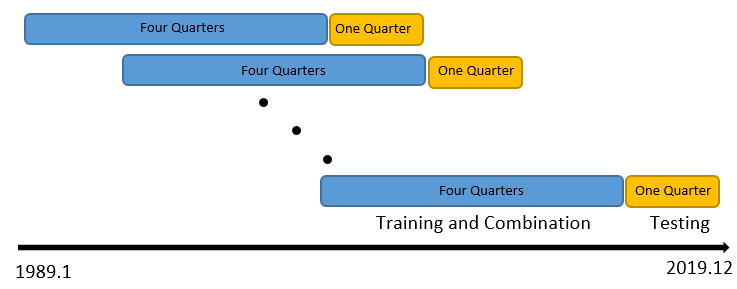
\includegraphics[scale=0.56]{rolling_windows}
In total, there are 120 rolling windows (30 years) examined in this analysis.
\end{block}
\end{frame}

\begin{frame}[t]{Rolling Sample Results}
\vspace*{-\baselineskip}
\begin{figure}
\caption{The RMSE of 120 Rolling Windows.}
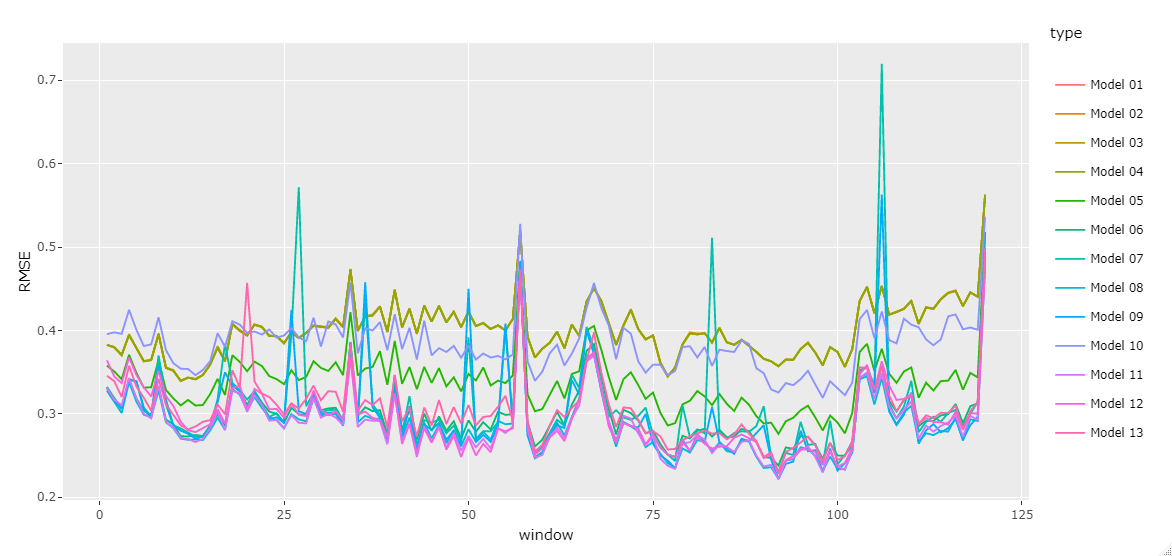
\includegraphics[scale=0.2]{rmse_rolling}
\end{figure}
\vspace*{-\baselineskip}
\begin{figure}
\caption{The MAPE of 120 Rolling Windows.}
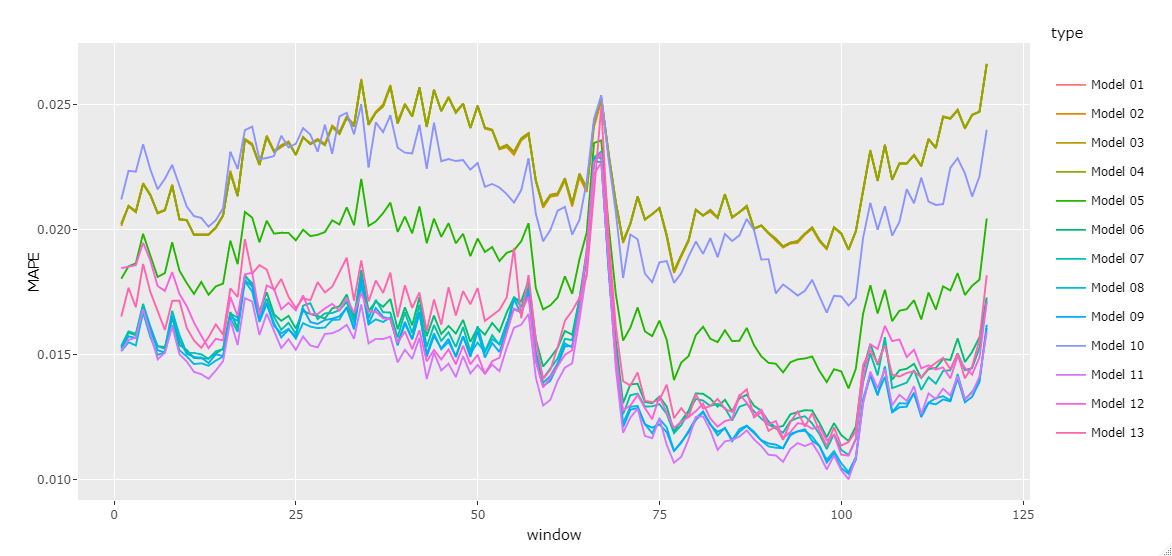
\includegraphics[scale=0.2]{mape_rolling}
\end{figure}

\end{frame}

\begin{frame}[t]{Rolling Sample Results Cont'd}

\begin{table}
\caption{Models Pick-up Rates in The 120 Rolling Windows (Full)}
\scalebox{0.66}{
\begin{tabular}{lccccccc}
Models &Intercept &Model 1 &Model 2 &Model 3 &Model 4 &Model 5 &Model 6\\
\hline
Frequency &\textcolor{red}{120} &99 &49 &62 &9 &55 &74\\
Percent &\textcolor{red}{100\%} &82.5\% &40.83\% &51.67\% &7.5\% &45.83\% &61.67\%\\
\hline
Models &Model 7 &Model 8 &Model 9 &Model 10 &Model 11 &Model 12 &Model 13\\
\hline
Frequency &65 &105 &104 &98 &\textcolor{red}{120} &\textcolor{red}{120} &77\\
Percent &54.17\% &87.5\% &86.67\% &81.67\% &\textcolor{red}{100\%} &\textcolor{red}{100\%} &64.17\%\\
\end{tabular}}
\end{table}
\vspace*{-\baselineskip}
\begin{block}
\noindent If past price joins the game, to resale observations, the past price is selected in \textcolor{blue}{119} windows; to first sale observations, the LASSO selection combination will rely on Random Forest and Boosting more. 
\end{block}

\end{frame}



\begin{frame}[t]{Rolling Sample Results Cont'd}

\begin{table}
\caption{Models Pick-up Rates in The 120 Rolling Windows (Past Price)}
\scalebox{0.66}{
\begin{tabular}{lccccccc}
Models &intercept &Model 1 &Model 2 &Model 3 &Model 4 &Model 5 &Model 6\\
\hline
Frequency &\textcolor{red}{120} &\textcolor{blue}{104} &20 &54 &6 &67 &55\\
Percent &\textcolor{red}{100\%} &\textcolor{blue}{86.67\%} &16.67\% &45\% &5\% &55.83\% &45.83\%\\
\hline
Models &Model 7 &Model 8 &Model 9 &Model 10 &Model 11 &Model 12 &Model 13\\
\hline
Frequency &57 &\textcolor{blue}{106} &\textcolor{blue}{108} &82 &\textcolor{red}{120} &\textcolor{red}{120} &85\\
Percent &47.5\% &\textcolor{blue}{88.33\%} &\textcolor{blue}{90\%} &68.33\% &\textcolor{red}{100\%} &\textcolor{red}{100\%} &70.83\%\\
\end{tabular}}
\end{table}

\begin{table}
\caption{Models Pick-up Rates in The 120 Rolling Windows (First Sale)}
\scalebox{0.66}{
\begin{tabular}{lccccccc}
Models &intercept &Model 1 &Model 2 &Model 3 &Model 4 &Model 5 &Model 6\\
\hline
Frequency &\textcolor{red}{120} &59 &37 &31 &5 &39 &53\\
Percent &\textcolor{red}{100\%} &49.17\% &30.83\% &25.83\% &4.17\% &32.5\% &44.17\%\\
\hline
Models &Model 7 &Model 8 &Model 9 &Model 10 &Model 11 &Model 12 &Model 13\\
\hline
Frequency &78 &73 &84 &76 &\textcolor{red}{119} &\textcolor{red}{120} &67\\
Percent &65\% &60.83\% &70\% &63.33\% &\textcolor{red}{99.17\%} &\textcolor{red}{100\%} &55.83\%\\
\end{tabular}}
\end{table}

\end{frame}


\begin{frame}[t]{Rolling Sample Results Cont'd}
\vspace*{-\baselineskip}
\begin{figure}
\caption{The Combination RMSE of 120 Rolling Windows.}
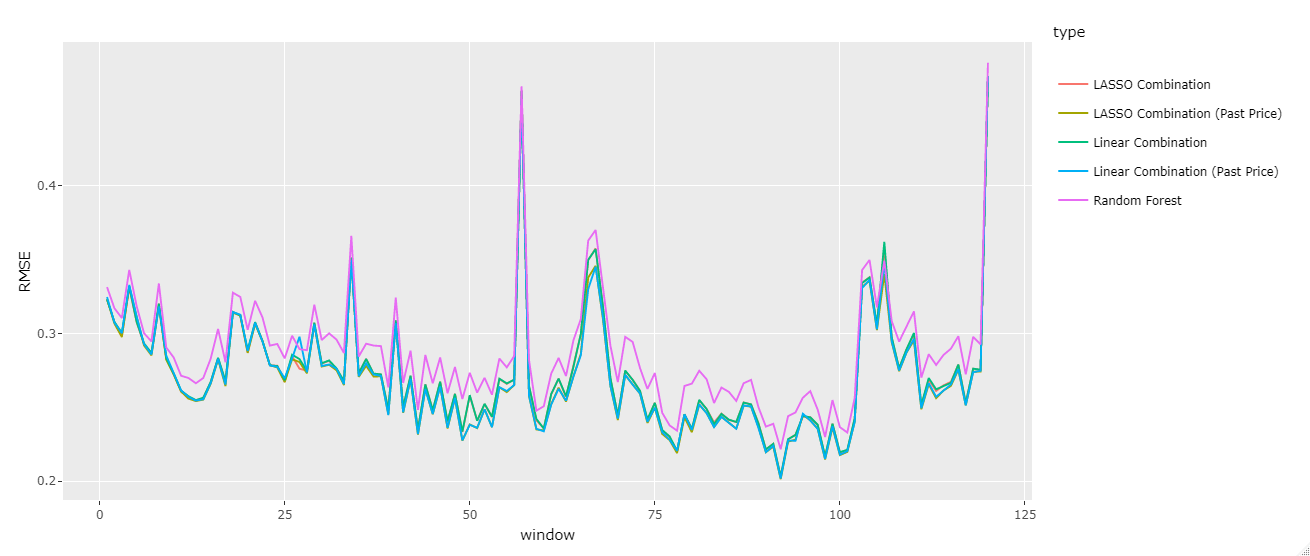
\includegraphics[scale=0.2]{rmse_combination_rolling}
\end{figure}
\vspace*{-\baselineskip}
\begin{figure}
\caption{The Combination MAPE of 120 Rolling Windows.}
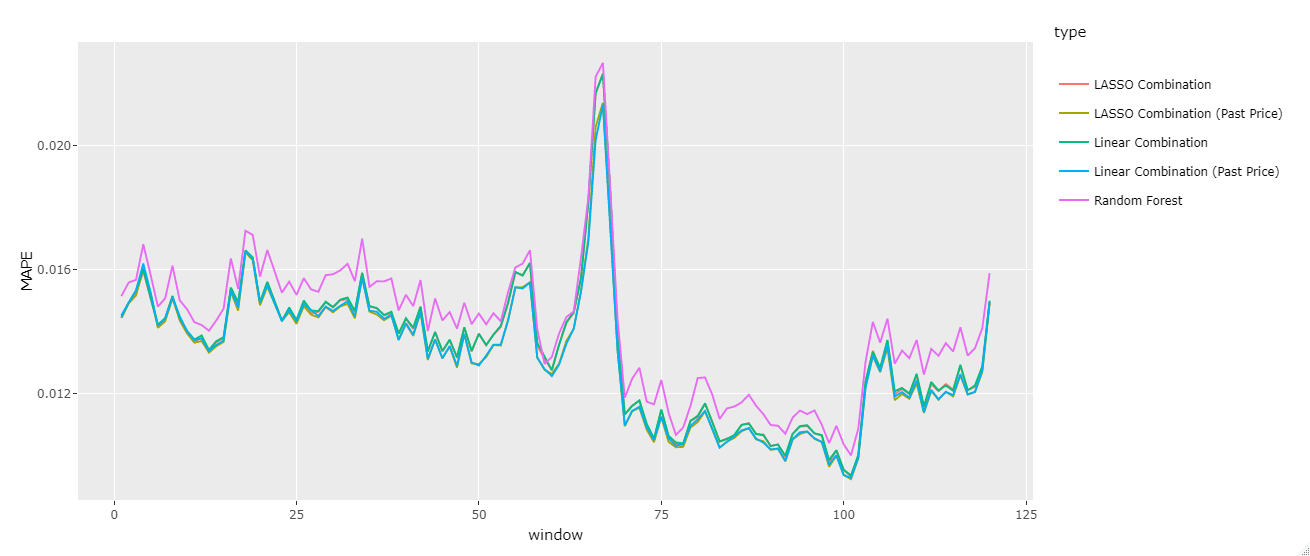
\includegraphics[scale=0.2]{mape_combination_rolling}
\end{figure}

\end{frame}


\section{Conclusions}

\begin{frame}[t]{Conclusions}

\begin{enumerate}
\item If just considering accuracy, the boosting model is the best. However, if interpretability is also a consideration, the spline model will be the most competitive one without doubts.
\item The combination provides a chance to the cooperation between models and other valuable information. This process can also increase the accuracy of prediction and reduce the uncertainty from models.
\item Some high accuracy models are consistently selected in the 120 rolling windows. Indirectly, it shows that the LASSO selection process works in the forecast combination, it gives similar accuracy comparing with linear combination by less variables. Also, in the rolling windows, it proves that no one can be survived in the huge market changes.  
\end{enumerate}

\end{frame}

\begin{frame}
\LARGE Thank you, any questions or comments?
\end{frame}




\end{document}